\usepackage[bib]{shared/cs45}

\title{CS 45, Lecture 2}
\subtitle{Shell Tools}
\date{Winter 2023}
\author{Akshay Srivatsan, Ayelet Drazen, Jonathan Kula}

\begin{document}

\maketitle

\frame{\titlepage}

\begin{frame}
  \frametitle{Outline}
  \tableofcontents[hidesubsections]
\end{frame}

\section{What is the Shell?}

To understand what the shell is, we first have to understand the environment in
which it was designed:

\begin{frame}{UNIX}
  \begin{itemize}
    \item
      The shell (as we recognize it) began with the UNIX \alert<2>{operating
      system} in 1969.\footcite{ritchie:unix}
    \item
      UNIX was made at Bell Labs by Ken Thompson and Dennis Ritchie.
    \item
      UNIX introduced what is now called \enquote{the UNIX philosophy.}
    \item
      Almost all modern computing is derived from the legacy of UNIX.
  \end{itemize}
\end{frame}

In fact, every currently-mainstream operating system has some of UNIX in it.
\textsc{macOS} is an actual descendant of UNIX (in particular, the Berkeley
Software Distribution, or BSD), and \textsc{Linux} is designed to be
UNIX-compatible, even though it was made independently. Even \textsc{Windows},
which historically held an entirely different philosophy and design, now
bundles a bundles a Linux compatibility layer, which transitively gives it UNIX
compatibility as well.

Now, we said UNIX is an \textsc{operating system}, but what exactly does that mean?

\subsection{What is an Operating System?}

An operating system, at its core, is an abstraction over the raw hardware of a
computer. A computer contains many different parts, each of which has a
different purpose:

\begin{frame}{Anatomy of a Computer}
  \pause
  \begin{description}
    \item[Input]
      Keyboards, Mice, \alert<8>{Serial Ports}, etc.\pause
    \item[Output]
      Screens, \alert<8>{Serial Ports}, Speakers, etc.\pause
    \item[Storage]
      Memory (RAM), Disks, Disc Readers, etc.\pause
    \item[Compute]
      CPUs (math), FPUs (math with decimals), GPUs (math with matrices)\pause
    \item[Networking]
      Ethernet, Wi-Fi, \alert<8>{Serial Ports}, etc.\pause
    \item[Misc.]
      Fans, Power Supplies, Sensors, etc.\pause\pause
  \end{description}
  \mode<article> {
    Different computers have different parts serving these purposes.  My
    laptop, for example, has very different hardware than the computer running
    \href{https://carta.stanford.edu}{Carta}.  However, they both use the same
    operating system kernel (i.e., Linux), and I can therefore run the same
    programs on both.
  }
  \begin{definition}[kernel]
    An \textsc{Operating System Kernel} is a program that abstracts over
    different hardware, allowing the same software to run on different
    computers.
  \end{definition}
\end{frame}

You might notice that \textsc{serial ports} show up quite a lot on this list.
At the time UNIX was designed, serial ports were ubiquitous---any time you
wanted to connect two devices together, you'd use a serial port.  Even today,
you can still see the legacy of serial ports hiding in the design of most
operating systems.

\begin{frame}{Userspace}
  \begin{itemize}
    \item
      A kernel by itself is kind of useless.\pause
    \item
      Abstractions are great, but we want to \textit{do} something with our
      computers.\pause
    \item
      This is where \textsc{userspace} comes in.\pause
  \end{itemize}
  \mode<presentation>{
    \vspace{1em}
  }
  \begin{definition}[userspace]
    \textsc{Userspace} is the set of programs that come bundled with an OS
    kernel, which allow a user to perform various tasks.
  \end{definition}
\end{frame}

Almost everything we'd call an ``program'' (or an ``app'') is a userspace
program.  While we can install programs/apps after-the-fact, every operating
system must come with some set of them installed; otherwise, the operating
system wouldn't be able to do anything.

\begin{frame}{Running Programs}
  \begin{itemize}
    \item
      Now that we have a bunch of programs installed, we want to run them.\pause
    \item
      We need something that wraps up all the programs and provides a common
      interface to them.\pause
  \end{itemize}
  \mode<article>{
    This common interface is what we call the \textsc{shell}.
  }
  \mode<presentation>{
    \vspace{1em}
  }
  \begin{definition}[shell]
    A \textsc{shell} is the outermost layer of an operating system; it lets a
    user run userspace programs, which in turn let a user interact with their
    computer's hardware.
  \end{definition}
  \pause
  \begin{definition}[operating system]
    An \textsc{Operating System} is the combination of a kernel, a set of
    userspace programs, and a shell.
  \end{definition}
\end{frame}

Modern operating systems have many different kinds of shells, depending on what
they're used for.  Some are graphical, some are text-based.  While graphical
ones are far more common for end-users, text-based ones are far more common for
developers.

\begin{frame}{Types of Shell}
  \only<4>{\vspace{-0.5em}}
  \begin{table}
    \centering
    \begin{tabular}{c|c|c|c}
      Operating System & Shell & Type & How you start programs \\
      \hline
      Windows & \texttt{explorer.exe} & Graphical & Start Menu, Desktop \\
      macOS & Aqua & Graphical & Dock, Launchpad \\
      iOS, Android & Home Screen & Graphical & Tap icon \\
      Linux & GNOME, KDE, XFCE, \ldots & Graphical & Various \\
      \hline
      \pause
      Windows & \texttt{cmd.exe} & Text & Type name of \texttt{.exe} file \\
      UNIX & \texttt{sh} & Text & \alert<2>{The rest of this lecture.} \\
      Linux & \texttt{bash} & Text & Same as \texttt{sh} \\
      macOS & \texttt{zsh} & Text & Same as \texttt{sh} \\
    \end{tabular}
    \caption{Shells across common operating systems}
    \label{tab:shells}
  \end{table}
  \mode<article>{
    Modern UNIX-like operating systems use more modern shells, like
    \texttt{bash} and \texttt{zsh}, but they're all backwards-compatible with
    the classic \texttt{sh}.  While \autoref{tab:shells} lists the default on each
    platform, some platforms let you change the default shell, and there are
    many \texttt{sh}-compatible shells available.

    Windows also has a more modern UNIX-shell derivative called
    \href{https://learn.microsoft.com/en-us/powershell/scripting/overview}{PowerShell},
    which is designed to be a hybrid of the traditional Windows command line,
    the UNIX shell, and Windows' native object-oriented interfaces.  It's not
    fully compatible with the UNIX shell, and is much less widely used, but
    it's worth checking out if you're curious about alternative shells; it has
    some cool features not found on traditional UNIX shells.
  }
  \pause
  While all of these shells can \textit{start} programs, only the UNIX shell
  (and its derivatives) can \textit{combine} them.%
  \mode<article>{%
    \footnote{%
      Okay, technically the other shells \textit{can} also combine programs to %
      some extent, but the UNIX shell can do so to a much greater extent.%
    }%

    This unique property, especially in combination with \textsc{The UNIX
    Philosophy}, has resulted in the UNIX shell growing into a powerful software
    ecosystem.
  }
\end{frame}

\subsection{The UNIX Philosophy}

The UNIX philosophy is a way of thinking about what a program should do.

\begin{frame}{Original}
  As described in the Bell System Technical Journal in 1978~\footcite{mcilroy:unix}:
  {
    \small
    \begin{enumerate}
      \item
        Make each program do one thing well. To do a new job, build afresh rather
        than complicate old programs by adding new "features."
      \item
        Expect the output of every program to become the input to another, as yet
        unknown, program. Don't clutter output with extraneous information. Avoid
        stringently columnar or binary input formats. Don't insist on interactive
        input.
      \item
        Design and build software, even operating systems, to be tried early,
        ideally within weeks. Don't hesitate to throw away the clumsy parts and
        rebuild them.
      \item
        Use tools in preference to unskilled help to lighten a programming task,
        even if you have to detour to build the tools and expect to throw some of
        them out after you've finished using them.
    \end{enumerate}
  }
\end{frame}

That's written very confusingly, but it's all just a really wordy way of saying:

\begin{frame}[c]{Simplified}
  \begin{block}{The UNIX Philosophy}
    Build lots of small tools, each of which does exactly one thing well, but
    which can be combined to do more powerful things.
  \end{block}
\end{frame}

The UNIX Philosophy is also deeply tied to the UNIX file abstraction.  Remember
how we said that the job of an OS kernel is to abstract over different
hardware?  Well, in UNIX (and UNIX-derived OSes):

\subsection{The UNIX File Abstraction}

\label{sec:unix_abstraction}
\begin{frame}{The UNIX File Abstraction}
  \begin{itemize}
    \item
      In UNIX, \alert<1>{everything is a file} (including hardware!).\pause
    \item
      Most files are text.\pause
    \item
      Programs which operate on text can operate on almost everything.
  \end{itemize}
  \mode<article>{
    The idea that \textit{everything is a file} is not an exaggeration.  Want
    to write to your screen?  Write to \texttt{/dev/fb} (the ``framebuffer'').
    Want to get input from the mouse?  Read from \texttt{/dev/input/mice}. Want
    to play a beep from the speaker?  Write to \texttt{/dev/snd/pcm*}. While
    this has reduced a bit on modern OSes, and there are now higher-level
    abstractions for many things, UNIX-based operating systems model an insane
    number of different things as files.
  }
\end{frame}

The combination of the UNIX Philosophy and the UNIX File Abstraction means we
have hundreds of small, single-purpose programs which operate on text files,
and we have every possible thing the computer could do represented as text
files.  The UNIX shell lets us combine these programs and these devices/text
files to do\ldots{} whatever we want, really.

\section{The UNIX Shell}

When you open the ``Terminal'' application on your computer, you'll be greeted
by the UNIX shell (from now on, just ``the shell''').\footnote{You can open the
\enquote{Terminal} application the same way you'd open a normal application; on
macOS it's located in the ``Utilities`` folder of ``Applications``, on Windows
it's in your start menu (it might be called ``Ubuntu``), and on Linux it'll be
in your desktop environment's normal app launcher.}

\begin{frame}{The UNIX Shell}
  \begin{center}
    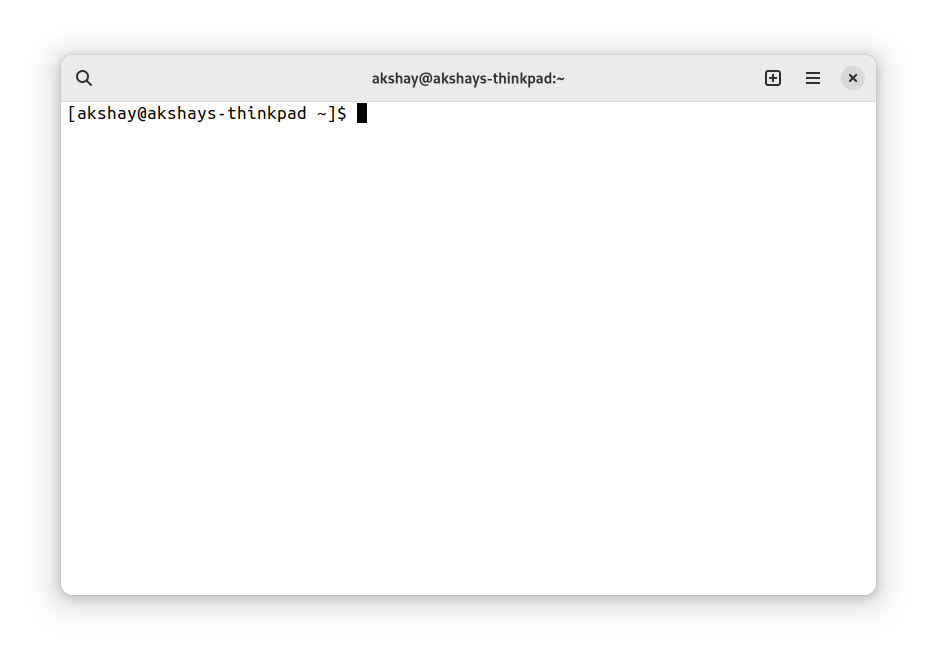
\includegraphics[width=0.5\paperwidth]{images/bash.png}
  \end{center}
\end{frame}

In particular, the shell will give you a ``prompt''; a sequence of information,
followed by a cursor where you can type commands.

\begin{frame}[fragile]{The Prompt}
  \begin{example}[prompt]
    An default shell prompt might look like this:
    \begin{minted}[escapeinside=||]{text}
[akshay@akshays-thinkpad ~]$ 
    \end{minted}
  \end{example}

  This \textsc{prompt} will print every time the shell is ready to accept
  another command.  It probably looks different on your computer, since
  different shells have different defaults.  Regardless of what it looks like
  right now, you can customize it to look like whatever you want.  In most
  cases, you can get back to it by pressing \textsc{CTRL-C} on your keyboard.

  \mode<article>{
    \begin{definition}[prompt]
      The prompt is a sequence of information printed by the shell when it's
      ready to accept a new command.
    \end{definition}
  }
\end{frame}

Let's look at the pieces of information in more detail:

\begin{frame}[fragile]{The Prompt}{Username}
  \begin{example}[prompt: username]
    This part of the prompt is your username:
    \begin{minted}[escapeinside=||]{text}
[|\color{red}akshay|@akshays-thinkpad ~]$ 
    \end{minted}
  \end{example}

  This is probably the same as the username you use to log into your computer.
  By default, you're auto-logged into the shell using your normal user account.
\end{frame}

\begin{frame}[fragile]{The Prompt}{Hostname}
  \begin{example}[prompt: hostname]
    This part of the prompt is your computer's hostname:
    \begin{minted}[escapeinside=||]{text}
[akshay@|\color{red}akshays-thinkpad| ~]$ 
    \end{minted}
  \end{example}


  This is your computer's name on whatever network it's connected to.
  Generally you don't really care about this unless you have multiple
  computers.
\end{frame}

\begin{frame}[fragile]{The Prompt}{Current Directory}
  \begin{example}[prompt: current directory]
    This part of the prompt is your current directory.
    \begin{minted}[escapeinside=||]{text}
[akshay@akshays-thinkpad |\color{red}~|]$ 
    \end{minted}
  \end{example}

  This is your \textsc{working directory}; \enquote{directory} is just a fancy
  name for \enquote{folder}, like you'd have in Windows Explorer or macOS Finder.

  \mode<article>{
    \begin{definition}[directory]
      A \textsc{directory} is a folder.  It can contain files and other
      directories.
    \end{definition}
    \begin{definition}[working directory]
      Your \textsc{working directory} is the directory you're \enquote{in};
      until you change your working directory, you can see only the files and
      folders in this directory.  This is also often called your
      \textsc{current directory}.  It can be abbreviated as \texttt{.}.
    \end{definition}

    Just like in Windows Explorer or macOS Finder, you're \enquote{in} a
    particular directory at any point in time, in which case you can see the
    files in that directory.
  }

  By default, you start in your \textsc{home directory}, which is the folder
  that contains \texttt{Documents}, \texttt{Downloads}, \texttt{Pictures},
  \texttt{Videos}, etc.  The home directory is abbreviated as a tilde
  (\textsc{\textasciitilde}) because it's so common.

  \mode<article>{
    \begin{definition}[home directory]
      Your \textsc{home directory} is the directory all your files are in.
      Everything \enquote{under} your home directory belong to you, while
      everything \enquote{above} it belongs to someone else (probably the OS
      itself).
    \end{definition}
  }
\end{frame}

The shell is a command interpreter: you type in commands, and it does them (or
gives you an error).  Unfortunately, the commands were all named half a century
ago when bytes were expensive, so the names cryptic and short.  Let's go
through a few useful commands to get started.

\section{Basic Commands}

\subsection{Directories}

\begin{frame}[fragile]{Listing Files}
  \mode<presentation>{
    \vspace{-0.5em}
  }
  In Windows Explorer or macOS Finder, the current directory is always visible.
  In the shell, you have to ask for the list of current files manually.

  \pause
  \alert<2>{The \textsc{list} command is called \texttt{ls}.}

  \pause
  \begin{example}[ls]
    On my computer, the results look like this:
    \begin{minted}{text}
[akshay@akshays-thinkpad ~]$ ls
Desktop    Downloads  Music     Public     Videos
Documents  Dropbox    Pictures  Templates
[akshay@akshays-thinkpad ~]$ 
    \end{minted}
  \end{example}
  These are all the \textsc{subdirectories} of my home directory.
  \mode<article> {
    \begin{definition}[subdirectory]
      A \textsc{subdirectory} is a directory contained within another
      directory.
    \end{definition}
  }
\end{frame}

\begin{frame}[fragile]{You are here}
  \begin{itemize}
    \item
      Before we go exploring, let's do one more command in the home directory.
  \end{itemize}
  \pause
  \alert<2>{The \textsc{print working directory} command is called \texttt{pwd}.}
  \pause
  \begin{example}[pwd]
    Print the current working directory:
    \begin{minted}{text}
[akshay@akshays-thinkpad ~]$ pwd
/home/akshay
[akshay@akshays-thinkpad ~]$ 
    \end{minted}
  \end{example}
  \pause
  \mode<article>{
    Note that \texttt{\textasciitilde} is actually short for
    \texttt{/home/akshay}.  Its \textsc{parent directory} is called
    \enquote{home}.  The parent directory of \enquote{home} doesn't have a name
    at all!

    \begin{definition}[parent directory]
      The \textsc{parent directory} of a subdirectory is the directory which
      contains the subdirectory.
    \end{definition}
  }

  \begin{definition}[root directory]
    The \textsc{root directory} is the topmost directory on the filesystem.  It's often called \texttt{/}.
  \end{definition}

  \mode<article> {
    \begin{definition}[filesystem]
      The \textsc{filesystem} is the hierarchy of directories which contain
      every file on your computer.  Some of these files are \enquote{real},
      i.e., they exist on your hard drive, and some are \enquote{virtual},
      i.e., they're made up by the OS kernel to represent hardware.
    \end{definition}
    N.B.: your computer might say something slightly different depending on
    your OS.  I think macOS would say \texttt{/Users/<username>}.
  }
\end{frame}

\begin{frame}[fragile]{Changing Directories}
  \begin{itemize}
    \item
      The home directory isn't too interesting on its own.
    \item
      Let's go somewhere you probably know well: the Desktop!
    \item
      In Explorer or Finder you could just click on a folder to enter it.
  \end{itemize}
  \pause
  \alert<2>{The \textsc{change directory} command is called \texttt{cd}.}
  \pause
  \begin{example}[cd]
    Change (\texttt{cd}) into the \texttt{Desktop} directory:
    \begin{minted}{text}
[akshay@akshays-thinkpad ~]$ cd Desktop
[akshay@akshays-thinkpad Desktop]$
    \end{minted}
  \end{example}
  \mode<article> {
    Note that my prompt changed to say \texttt{Desktop} instead of
    \texttt{\textasciitilde}.
  }
\end{frame}

\begin{frame}[fragile]{Not Changing Directories}
  \begin{itemize}
  \item
    There's a special name that always means \enquote{the current directory}: \mintinline{text}{.}
  \item
    \mintinline{text}{cd .} says \enquote{change directory to the current directory}.
  \end{itemize}
  \pause
  \begin{example}[cd .]
    Don't change directories:
    \begin{minted}{text}
[akshay@akshays-thinkpad Desktop]$ pwd
/home/akshay/Desktop
[akshay@akshays-thinkpad Desktop]$ cd .
[akshay@akshays-thinkpad Desktop]$ pwd
/home/akshay/Desktop
    \end{minted}
  \end{example}
  \mode<article> {
    From now on, I'm going to omit the part of the prompt before the
    \texttt{\$} because it's not very useful for our purposes, and it varies
    from computer to computer anyway.
  }
\end{frame}

\begin{frame}[fragile]{Making Directories}
  \mode<presentation>{\vspace{-1em}}
  \begin{itemize}
    \item
      Now that we're on the desktop, let's create a new directory to do some
      experiments in.
    \item
      This is the equivalent of right-clicking and selecting \enquote{New Folder}.
  \end{itemize}
  \pause
  \alert<2>{The \textsc{make directory} command is called \texttt{mkdir}.}

  \pause
  \begin{example}[mkdir]
    Create a directory called \enquote{cs45-test-directory} and \texttt{cd} into it:
    \begin{minted}{text}
$ mkdir cs45-test-directory
$ cd cs45-test-directory/
    \end{minted}
  \end{example}
  You can go back to the Desktop by typing \mintinline{shell}{cd ..} or
  \mintinline{shell}{cd ~/Desktop}.

  \mode<article>{
    In general, \mintinline{shell}{..} is a special name which always refers to
    the parent of the current directory. Regardless of where you are, you can
    always go to the parent directory by typing \mintinline{shell}{cd ..}.

    Now that we can make directories, you might be wondering how to delete
    them.  The process is actually almost the same, just with a different
    command.
  }
  \pause
  \alert{The \textsc{remove directory} command is \texttt{rmdir}.}

  \mode<article>{
    This is used almost the same way as mkdir; one thing to note is that
    \texttt{rmdir} can only be used on an empty directory.
  }
\end{frame}

Let's review what we've covered about directories:

\begin{frame}[c]{Directory Review}

  \mode<presentation> {
    \vspace{-0.75em}
  }

  \begin{table}
    \centering
    \begin{tabular}{c|c}
      Shortcut & Name\\
      \hline
      \texttt{\textasciitilde} & Home Directory \\
      \texttt{/} & Root Directory \\
      \texttt{.} & Current Directory \\
      \texttt{..} & Parent Directory \\
    \end{tabular}
    \caption{Directory Shortcuts}
    \label{tab:dir_shortcuts}
  \end{table}

  \pause

  \begin{table}
    \centering
    \begin{tabular}{c|c|c|c}
      Command & Description & Argument & Required \\
      \hline
      \texttt{ls} & List Directory & Directory Name & No, defaults to \texttt{.} \\
      \texttt{cd} & Change Directory & Directory Name & No, defaults to \texttt{\textasciitilde} \\
      \texttt{pwd} & Print Working Directory & N/A & N/A \\
      \texttt{mkdir} & Make Directory & Directory Name & Yes \\
      \texttt{rmdir} & Remove Directory & Directory Name & Yes \\
    \end{tabular}
    \caption{Directory Commands}
    \label{tab:dir_commands}
  \end{table}

  \mode<article> {
    \begin{definition}[argument]
      An \textsc{argument} is an input provided to a command.  This may be a
      filename or arbitrary text, depending on the command.  It is passed to a
      command by specifying it after the command name.  By default, arguments
      are separated by spaces; if you want to provide an argument with a space,
      use double- or single-quotes around the argument.
    \end{definition}
  }
\end{frame}

\subsection{Files}

Now that we can create, delete, and move around directories, let's start
working with files.  As mentioned in \autoref{sec:unix_abstraction}, everything in
UNIX is a file, so (in a way) we're actually learning to work with
\textit{everything}.

However, before we work with files, let's take a brief diversion to look at
something a little more basic: input/output.

\begin{frame}[fragile]{Output}
  \begin{itemize}
    \item
      Sometimes we just want to print something out, like \enquote{hello,
      world}.
  \end{itemize}
  \pause
  \alert<2>{The \textsc{print} command is called \texttt{echo}}.
  \pause
  \begin{example}[echo]
    Print the text \enquote{hello, world}:
    \begin{minted}{text}
$ echo "hello, world"
hello, world
$ 
    \end{minted}
  \end{example}
\end{frame}

The name \enquote{echo} is a bit less intuitive than the ones we've seen
before, but it makes sense: it \enquote{echoes} back anything you tell it.

If you're familiar with programming in C, you might also like the \textsc{print
formatted} command, \texttt{printf}.  You can use it the same way as the C
\texttt{printf} function, except you don't need parentheses.

\begin{example}[printf]
  Print the text \enquote{hello, world} using \texttt{printf}:
  \begin{minted}{text}
$ printf "%s, %s\n" "hello" "world"
hello, world
$ 
  \end{minted}
\end{example}

\begin{frame}[fragile]{Input}
  \only<1-3>{
    \begin{itemize}
      \item
        Sometimes we want to read input from the user.
        \pause
      \item
        Unfortunately, this is trickier: there are multiple commands which can be
        used for input.  Let's use the simplest one.
    \end{itemize}
  }
  \pause
  \only<presentation|4->{
    \vspace{-1em}
  }
  \alert<3>{The \textsc{concatenate} command is called \texttt{cat}}. It can
  also be used for input.
  \pause
  \begin{example}[cat]
    Read text from the user:
    \begin{minted}{text}
$ cat
this is a test
this is a test
line 2
line 2
$ 
    \end{minted}
  \end{example}

  The \texttt{cat} command will print out whatever you type into it\ldots~
  forever.  To get it to stop, you can either \enquote{kill} it by pressing
  \textsc{CTRL-C}, or tell it \enquote{end of file} by pressing
  \textsc{CTRL-D}.
  \mode<article> {
    Note that this is actually the \textsc{control} key, even on Macs.  Using
    the \textsc{command} key will not work.

    Aside: Windows and Linux users might be wondering how you copy and paste from the
    terminal if \textsc{CTRL-C} kills programs instead of copying anything. The
    answer is: it's complicated. The UNIX shell predates \textsc{CTRL-C} and
    \textsc{CTRL-V} for copy-and-paste, so they use those shortcuts for other
    things.  Different terminal emulators (the program called
    \enquote{Terminal} on your computer) have different ways of doing
    copy-and-paste; mine uses \textsc{CTRL-SHIFT-C} and \textsc{CTRL-SHIFT-V},
    but yours might use something else.  Mac users don't have to worry about
    this, since they can use \textsc{CMD-C} and \textsc{CMD-V} as usual.
  }
\end{frame}

Enough on I/O (as input/output is often called); let's get back to files.

\begin{frame}[fragile]{Creating Files}
  \begin{itemize}
    \item
      There are a few different ways to create files.  Let's start with the
      simplest.
  \end{itemize}
  \pause
  \alert<2>{The \textsc{touch file} command is called, intuitively,
  \texttt{touch}.}  While we don't care about \enquote{touching} files as such,
  it has the handy side effect of creating files.\mode<article>{%
    \footnote{
      \enquote{Touching} a file means changing its last-modified timestamp to
      the current time; essentially like opening a file, saving it, and closing
      it again.  This isn't useful very often, so most people think of
      \texttt{touch} as the \enquote{create file} command.
    }
  }
  \pause
  \begin{example}[touch]
    To create a file called \enquote{text.txt}:
    \begin{minted}{text}
$ touch test.txt
$ ls
test.txt
$
    \end{minted}
  \end{example}
\end{frame}

We can also rename or move the file we just created.

\begin{frame}[fragile]{Renaming Files}
  \alert<1>{The \textsc{move file} command is called \texttt{mv}.}  It can also
  be used to rename files.  \pause
  \begin{example}[mv]
    To rename a file called \enquote{text.txt} to \enquote{empty.txt}:
    \begin{minted}{text}
$ mv test.txt empty.txt
$ ls
empty.txt
$
    \end{minted}
  \end{example}
\end{frame}

\begin{frame}[fragile]{Deleting Files}
  \alert<1>{The \textsc{remove file} command is called \texttt{rm}.}
  \begin{alertblock}{This is irreversible!}
    This command is dangerous!  It does \textbf{not} move the file to a
    \enquote{trash} folder; it permanently and irreversibly deletes it.
  \end{alertblock}\pause
  \begin{example}[rm]
    To remove a file called \enquote{text.txt}:
    \begin{minted}{text}
$ rm test.txt
$
    \end{minted}
  \end{example}
\end{frame}

\begin{frame}[fragile]{Writing to Files}
  \only<presentation|3->{\vspace{-0.5em}}
  \begin{itemize}
    \item
      We have a problem though: the file we created is empty.  We can't do much
      with a bunch of empty files.
    \item
      We can check this by running \texttt{ls} with a special \textsc{flag}
      asking for extra info (including the file size).
  \end{itemize}
  \mode<article> {
    \begin{definition}[flag]
      A \textsc{flag} is a special argument to a function which configures its
      behavior.  By convention, flags can be short (a single letter) or long (a
      word), and start with either one or two hyphens to distinguish them from
      normal arguments.
    \end{definition}
  }
  \pause
  \begin{example}[ls -l]
    To print extra information about files:
    \begin{minted}[escapeinside=||]{text}
$ ls -l
total 0
-rw-r--r-- 1 akshay akshay |\color{red}0| Dec 18 11:59 test.txt
    \end{minted}
  \end{example}
  \mode<article>{
    This prints out a bunch of information we don't really care about right
    now: the file permissions, the file's owner, the file's group, and the
    file's last-modified time.  What we do care about is the \enquote{0}
    highlighted in red above: the file is zero bytes long.

    As an aside, the real purpose of the \texttt{touch} command we just used is
    to update the modification time of the file.  If you touch the file and run
    \texttt{ls -l} again, you should see the last-modified time update.
  }
  \pause
  \alert<presentation>{One very useful flag which is supported by almost every
  command is \texttt{--help}.}%
  \mode<article>{ %
    This will usually print out information about how to use that command.  On
    some commands the short form \texttt{-h} will also work, but that's
    sometimes used for something else.
  }
\end{frame}

\begin{frame}[fragile]{Writing to Files}
  \begin{itemize}
    \item
      Everything is a file, including the output of our commands.
      \pause
    \item
      By default, this is called \textsc{standard output}, and goes to our
      terminal.
      \pause
    \item
      The shell lets us \textsc{redirect} standard output to go to a file
      instead.
  \end{itemize}
  \pause
  \begin{example}[output redirection]
    To create a file called \enquote{hello.txt} with the contents
    \mintinline{text}{hello, world}:
    \begin{minted}{text}
$ echo "hello, world" > hello.txt
$
    \end{minted}
    To append to an existing file, you can use \mintinline{text}{>>} instead of
    \mintinline{text}{>}.
  \end{example}
\end{frame}

\begin{frame}[fragile]{Reading from Files}
  \begin{itemize}
    \item
      Just like \textsc{standard output}, the input to our programs is also a
      file.
      \pause
    \item
      By default, this is called \textsc{standard input}, and comes from our
      terminal.
      \pause
    \item
      The shell also lets us \textsc{redirect} standard input to come from a
      file.
  \end{itemize}
  \pause
  \begin{example}[input redirection]
    To print a file called \enquote{hello.txt}:
    \begin{minted}{text}
$ cat < hello.txt
hello, world
$
    \end{minted}
  \end{example}
  \mode<article>{
    This is actually slightly redundant, since the \texttt{cat} command lets us
    specify a specific file to use as input directly, so \mintinline{text}{cat
    hello.txt} would do the exact same thing.  The redirection approach is more
    general though: it works with any command that accepts input.
  }
\end{frame}

When the shell runs a program, it sets up its input and output using special
files.\footnote{
  Technically, these are \textsc{file descriptors} rather than files, but the
  distinction isn't very important for this class so we're glossing over it. If
  you're interested in learning more, come talk to us or take
  \href{https://cs111.stanford.edu}{CS111}.
}

\begin{frame}[c]{I/O(/E?)}
  \begin{definition}[standard input]
    \textsc{Standard input} (\texttt{/dev/stdin}) is the file from which a
    program reads its input.  
  \end{definition}
  \begin{definition}<2->[standard output]
    \textsc{Standard output} (\texttt{/dev/stdout}) is the file to which a
    program writes its output.
  \end{definition}
  \begin{definition}<3->[standard error]
    \textsc{Standard error} (\texttt{/dev/stderr}) is the file to which a
    program writes its error messages.
  \end{definition}
\end{frame}

Since these files are so widely used, the shell provides easy ways to redirect
them.  We've already seen a few of these.

\begin{frame}[c]{Redirection Operators}
  \begin{table}
    \centering
    \begin{tabular}{c|c|c}
      Operator & File & Overwrite? \\
      \hline
      \texttt{<} & \texttt{/dev/stdin} &  \\
      \texttt{>} & \texttt{/dev/stdout} & Overwrite \\
      \texttt{>>} & \texttt{/dev/stdout} & Append \\
      \texttt{2>} & \texttt{/dev/stderr}\footnote{It's uncommon to redirect standard error, but there are some valid reasons to (which we'll see later in the quarter).} & Overwrite \\
      \texttt{2>>} & \texttt{/dev/stderr} & Append \\
    \end{tabular}
    \caption{UNIX Shell Redirection Operators}
    \label{tab:redirection}
  \end{table}
\end{frame}

You might have seen the \texttt{>} operator before, in the form
\mintinline{shell}{> /dev/null}.  \texttt{/dev/null} is a special file that
discards anything written to it, so it's common to use it when the output of a
command is unimportant.

As it turns out, if we're doing multiple commands in a sequence, we don't even
need to write the results out to a file until the very end---we can use
\textsc{pipes} to send the output of one command directly into another command.

\section{Pipes}

\begin{frame}[fragile]{Environment Variables}
  Some programs need configuration that's too annoying to provide as arguments
  every time.
  \pause
  \begin{definition}[environment variable]
    An \textsc{environment variable} is a configuration value that's set
    globally by a program, which applies to itself and any other programs it
    runs.
  \end{definition}
\end{frame}

We'll talk about environment variables some more in \textit{Lecture 5: Command
Line Environment}.  For now, we just need to know that they exist and are
widely used.

\begin{frame}[fragile]{All the Environment Variables}
  \mode<presentation>{
    \vspace{-1em}
  }
  \alert<1>{The \textsc{environment variable} command \texttt{env} prints all the
  environment variables which are currently set.}
  \pause
  \begin{example}[env]
    To print every environment variable:
  \begin{minted}{text}
$ env
MAIL=/var/spool/mail/akshay
PWD=/home/akshay
XDG_SESSION_TYPE=wayland
PATH=/usr/local/bin:/usr/bin:/usr/local/sbin
HOME=/home/akshay
USERNAME=akshay
[...]
  \end{minted}
  \end{example}
  \mode<article>{
    This is quite long on my computer\ldots
  }
\end{frame}

\begin{frame}[fragile]{Pipes}
  \begin{itemize}
    \item
      Let's see how many environment variables we have!
      \pause
    \item
      \alert<2>{The \textsc{word count} command is called \texttt{wc}.}
      \pause
    \item
      It has a flag \texttt{--lines} (or \texttt{-l}) which counts lines in its
      input instead of words.
      \pause
  \end{itemize}
  \mode<article>{
    Now, there's two ways we could get the output of \texttt{env} into \texttt{wc}.
  }
  \begin{example}<only@4>[count environment variables with a temporary file]
    We can write the output into a temporary file, and give it as input to
    \texttt{wc}:
  \begin{minted}{text}
$ env > /tmp/env.txt
$ wc --lines < /tmp/env.txt
78
  \end{minted}
  \end{example}
  \mode<article>{
    This is kind of annoying though\ldots we need to do two separate commands,
    and we need to create a temporary file somewhere.

    As an aside, it's conventional to put temporary files in \texttt{/tmp}.
    Most systems will keep \texttt{/tmp} entirely in RAM, so any files there
    will automatically get deleted when you reboot.

    However, we can actually do this in a one-liner, without needing any
    temporary files at all.
  }
  \pause
  \begin{example}<only@5>[count environment variables with a pipe]
    We can connect the output of \texttt{env} and the input of \texttt{wc} with
    a \textsc{pipe}:
  \begin{minted}{text}
$ env | wc --lines
78
  \end{minted}
  \end{example}
\end{frame}

\begin{frame}{Benefits of Pipes}
  \begin{definition}[pipe]
    A \textsc{pipe} is a direct connection between the output of one program
    and the input of another.  It can be set up using the \texttt{|} (pipe)
    operator, which connects \texttt{stdout} of whatever is on the left with
    \texttt{stdin} of whatever is on the right.
  \end{definition}
  \pause
  Pipes are superior to temporary files for several reasons:
  \pause
  \begin{itemize}
    \item
      They are \textbf{parallel}: the programs on the left and right can run at
      the same time.
      \mode<article> {
        This is especially useful when the programs need to do lots of
        computation or external I/O; the right-side program can process the
        data it has already read, while the left-side program is waiting for or
        computing data to write.
      }
      \pause
    \item
      They are \textbf{lazy}: the program on the right can read exactly as much data as it needs from the program on the left.
      \mode<article>{
        In many cases, the right-side program may only need part of its input,
        in which case the left-side program doesn't need to compute the rest.
        This is especially useful when the left-side program is infinite or
        long-lived.
      }
  \end{itemize}
\end{frame}

\begin{frame}[c,fragile]{More Piping}
  \begin{example}<only@1>[the first $n$ environment variables]
    With the \texttt{head} command, we can extract only the first few lines
    from a file:
    \begin{minted}{text}
$ env | head --lines=3
MAIL=/var/spool/mail/akshay
PWD=/home/akshay
XDG_SESSION_TYPE=wayland
$
    \end{minted}
  \end{example}

  \pause
  \begin{example}<only@2>[random numbers]
    We can lazily evaluate part of an infinitely long \enquote{file} such as
    \texttt{/dev/random}:
    \begin{minted}{text}
$ cat /dev/random | hexdump | head --lines 1
0000000 4730 003c 6c22 1d16 49ef 6eff 91b2 a9f0
    \end{minted}
  \end{example}
\end{frame}

\section{Conclusion}
\begin{frame}{Getting Help}
  \begin{itemize}
    \item
      The shell is far more complicated than we can possibly cover in an
      80-minute lecture.
      \pause
    \item
      Most commands have lots of flags and options.
      \pause
    \item
      We already talked about the \texttt{--help} flag, which usually gives you
      a brief summary of how to use a command.
  \end{itemize}
\end{frame}

\begin{frame}[fragile]{The System Manual}
  \begin{itemize}
    \item
      One super-useful resource is the UNIX system manual, which is
      pre-installed on most UNIX-like systems.
      \pause
    \item
      \alert<2>{The \textsc{manual} command is \texttt{man}}; it takes as an
      argument the name of a command, and it displays the manual page
      (\enquote{man page}).
      \pause
    \item
      If you don't know the name of a command, you can search the manual using
      the command \texttt{apropos} (or, equivalently, \texttt{man --apropos}).
  \end{itemize}
  \pause
  \begin{example}<only@4>[man wc]
    To open the UNIX manual page for the \texttt{wc} word-count tool:
    \begin{minted}{text}
    $ man wc
    \end{minted}
  \end{example}
  \pause
  \begin{example}<only@5>[man man]
    To open the UNIX manual page for the manual itself:
    \begin{minted}{text}
    $ man man
    \end{minted}
  \end{example}
\end{frame}

Man pages open in what's called a \textsc{pager}; this is a program that makes
a long file readable on a short terminal.  You start at the beginning of the
file, and you can scroll up or down using the arrow keys.  You can quit by
pressing \texttt{q}.

\begin{frame}{To be continued\ldots}
  \begin{itemize}
    \item
      We'll continue exploring shell tools in Lecture 3: \textit{Data
      Manipulation and Shell Scripting}.
      \pause
    \item
      There's no class on Monday, January 16th (Martin Luther King Jr. Day);
      we'll pick back up on \alert<2>{Wednesday, January 18th}.
      \pause
    \item
      We'll post Assignment 1 soon, but it'll only be due on Monday, January
      23rd (twelve days from now).  It'll cover Lectures 2 (this one) and 3
      (next week).
  \end{itemize}
\end{frame}

\begin{frame}{To be continued\ldots{ }(Continued)}
  \begin{itemize}
    \item
      In the meantime: try doing file management from the terminal.  We didn't
      cover every command you'll need, so if you don't know how to do
      something, try searching the manual using \texttt{apropos} or searching
      the web.
      \pause
    \item
      Take a look at the UNIX filesystem hierarchy layout, documented in
      \texttt{man hier}. \mode<article>{You don't have to understand everything
      in there (lots of it is archaic/irrelevant to modern PC usage), but it's
      good to know roughly what's stored where.}
    \item
      Use \texttt{man} pages, \url{http://cheat.sh/}, or
      \url{https://devhints.io/bash} to find out more about shell commands.
  \end{itemize}
  \pause
  \begin{alertblock}{Be Careful!}
    The shell often doesn't warn you when you're doing dangerous things!  Be
    sure to read the \texttt{man} page before running commands you find on the
    internet.  Be especially careful with the \textsc{remove file} command,
    \texttt{rm}, or when using the \texttt{>} (overwrite) operator.
  \end{alertblock}
\end{frame}

Normally, most OS-critical files on your computer are protected using
\textsc{file permissions}, which we'll learn about in Lecture 5.  However,
there's a special command (which we saw briefly on Monday) which can override
file permissions and do potentially catastrophic things.

\begin{frame}{Sudo}
  \begin{alertblock}{Using \texttt{sudo} responsibly}
    \begin{itemize}
      \item
        Some commands require the use of \texttt{sudo}, the \textsc{superuser
        do} command.
      \pause
      \item
        This gives that command full access to do anything on your computer!
      \pause
      \item
        Sometimes \texttt{sudo} won't even ask for your password!
      \pause
      \item
        If you're using \texttt{sudo}, make sure you know what the command
        after it will do.
      \pause
      \item
        \texttt{sudo} is necessary for certain tasks (we'll see some in the
        next few lectures), but it's always good to be careful around it.
    \end{itemize}
  \end{alertblock}
\end{frame}

\begin{definition}[superuser]
  The \textsc{superuser} is a special account, often called the \textsc{root
  account}, with full power over a UNIX system.\footnote{
    Recent versions of macOS have an extra layer of protection, called
    \enquote{System Integrity Protection}, that stops even the superuser from
    doing \textit{really} dangerous things.  However, the superuser can still
    do a lot of things an ordinary user cannot.
  }  They are the equivalent of the Windows Administrator account.  Some
  regular accounts, called \enquote{sudoers}, have the ability to act as the
  superuser using the \texttt{sudo} command.
\end{definition}

And it's not just me who thinks that \texttt{sudo} can be dangerous, the first
time you run \texttt{sudo} it'll give you a warning about how dangerous it is:

\begin{frame}[fragile]{Sudo Warning}
  \begin{minted}{text}
  We trust you have received the usual lecture from the local System
  Administrator. It usually boils down to these three things:

      #1) Respect the privacy of others.
      #2) Think before you type.
      #3) With great power comes great responsibility.
  \end{minted}
\end{frame}

All that said, there are legitimate reasons to use \texttt{sudo} (for example,
installing software).  Just be careful around it, and don't run commands as
\texttt{sudo} just because you got a \enquote{permission denied} error; make
sure there \textit{is} a reason you have to use \texttt{sudo}.

Here are a few interesting commands to look up/try out before next class; try
looking up their \texttt{man} pages and how to use them:

\begin{frame}{Interesting Commands}
  \begin{description}
    \item{\texttt{head}:} Get the beginning of a file (or pipe).
    \item{\texttt{tail}:} Get the end of a file (or pipe).
    \item{\texttt{grep}:} Search within a file.
    \item{\texttt{sed}:} Find-and-replace.
    \item{\texttt{cut}:} Get a specific \enquote{column} of a file (e.g., a CSV file).
    \item{\texttt{ping}:} Test your internet connection.
    \item{\texttt{sort}:} Sort lines in a file.
    \item{\texttt{uniq}:} Remove duplicate lines in a file.
    \item{\texttt{exit}:} Exit the terminal.
  \end{description}
\end{frame}

Note that \texttt{uniq} requires its input to be sorted; it's not super clear
why the authors made this decision, it's generally good practice to pipe
through \texttt{sort} before piping into \texttt{uniq}.

\begin{frame}{Questions?}
  \begin{center}
    
\includegraphics[width=0.75\paperwidth]{images/unix-system.png}
  \end{center}
\end{frame}

\mode<article>{
  \newpage
  \bibliographystyle{plain}
  \bibliography{shared/cs45}
}

\mode<presentation>{
  \begin{frame}{References}
    \bibliographystyle{plain}
    \bibliography{shared/cs45}
  \end{frame}
}

\end{document}
